\documentclass[a4paper]{article}

\usepackage[utf8]{inputenc}

\usepackage{url}
\usepackage[hidelinks]{hyperref}

\usepackage{caption}

\usepackage{listings}

\usepackage{color}

\usepackage{enumitem}

% *** GRAPHICS RELATED PACKAGES ***
%\usepackage[pdftex]{graphicx}
\usepackage{graphicx}
%\usepackage[dvips]{graphicx}
% to place figures on a fixed position
\usepackage{float}

\usepackage[margin=1in]{geometry}

\title{IoT Lab}
\author{}
\date{}


\begin{document}

\maketitle

\tableofcontents

\section{IoT lab measurement exercises}

In the first phase of the lab a micro-controller will be transformed into a mote. A sensor mote is capable of detect various parameters of its environment and is capable of communication. For this purpose a sensor and a radio module is going to be attached to the micro-controller. For this same device an actuator is going to be connected to it. Furthermore a simple display device is also connected to the already built hierarchy.

In the second phase of the lab a virtual device is created using one of the cloud IoT provider's services that is going to accept and process the data arriving from our physical sensor. The service is going to store and display the data. Furthermore a virtual controller is attached to the virtual sensor that is going to send control signals for the physical device. A gateway device is used for translating the data into the right format between the physical and virtual devices.

The arrangement of these components can be seen on Figure~\ref{fig:meas-arrangement}. The task of the students attending this lab is to program the devices and the gateway for the achieving the desired operation.

\begin{figure}[H]
    \centering
    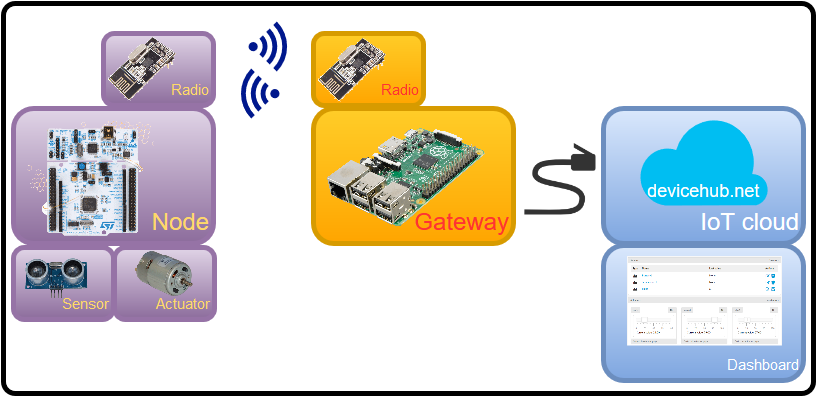
\includegraphics[width=0.9\textwidth]{figures/devices-arrangement.png}
    \caption{Arrangement of devices and components used in this lab}
    \label{fig:meas-arrangement}
\end{figure}

During the exercises a lab report has to be created. In this report the students must document the actions carried out, the code written, the configuration files created etc. The lab report can also contain screen captures. The basic guideline is to create such a document of which the measurement is easily reproducible. 

\section{Getting started with \emph{\textbf{mbed}} environment}

mbed is an IDE (and also an operating system) tailored for IoT applications based 32 bit ARM micro-controllers. There are several commercially available boards available as a result it allows simple and rapid prototyping. One of its main advantages compared to other IDEs that it can handle multiple types of micro-controllers so that the code written can be reused in multiple environments. Furthermore its UI is intuitive and also supports on-line workflows with team integration and version control. Naturally there are some cons as well namely that from mbed the low-level hardware components are not reachable from it and sometimes the basis of the framework called \emph{mbed OS} might contain bugs.

The micro-controller used during this lab is of type NUCLEO-F446RE.

\subsection{First steps}

Before proceeding any further register on site \url{https://developer.mbed.org/}. The registration is simple and easy and doesn't require instant verification of our e-mail addresses. After successful registration log-in on the website and then
\begin{enumerate}
  \item Go to ``Platforms" tab where the development board is selected
  \item Filter the results for manufacturer of "STMicroelectronics"
\end{enumerate}
\begin{figure}[H]
    \centering
    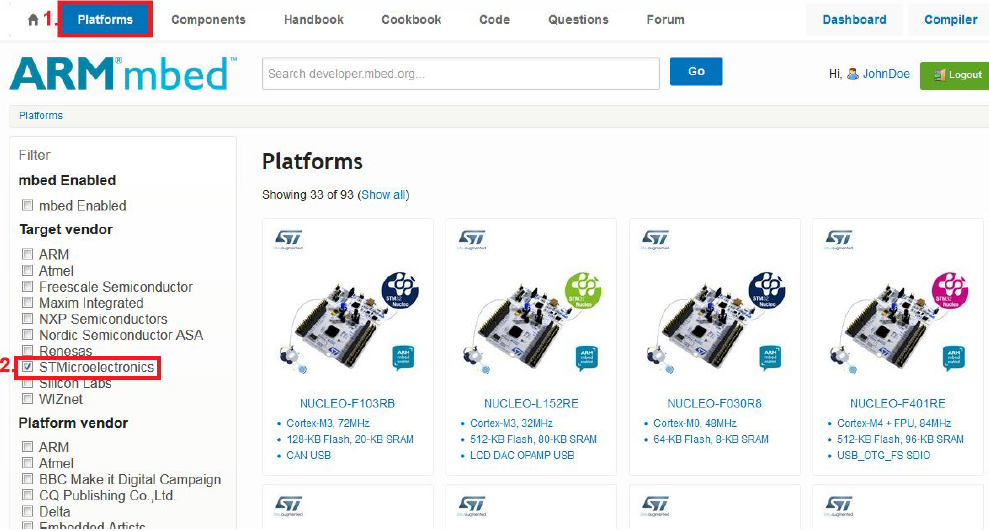
\includegraphics[width=0.9\textwidth]{figures/mbed-platform.png}
\end{figure}
\begin{enumerate}[resume]
\item Search for and select ``NUCLEO-F446RE" dev board. Here we can find detailed description on the micro-controller and also the schematics for the pin to feature connector assignment and functions associated with them
\end{enumerate}
\begin{figure}[H]
    \centering
    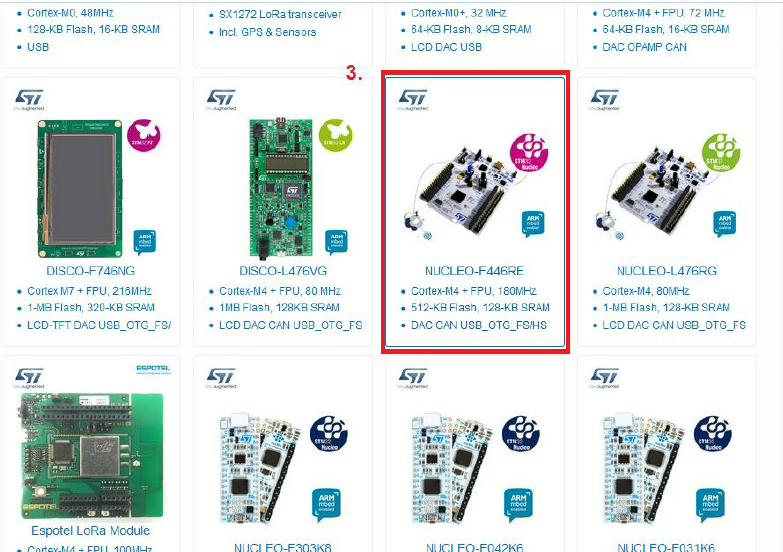
\includegraphics[width=0.9\textwidth]{figures/mbed-nucleo.png}
\end{figure}
\begin{enumerate}[resume]
\item Add the selected board to the compiler by clicking on the ``Add to your mbed Compiler" and the open it using the link in the upper right corner (5.)
\end{enumerate}
\begin{figure}[H]
    \centering
    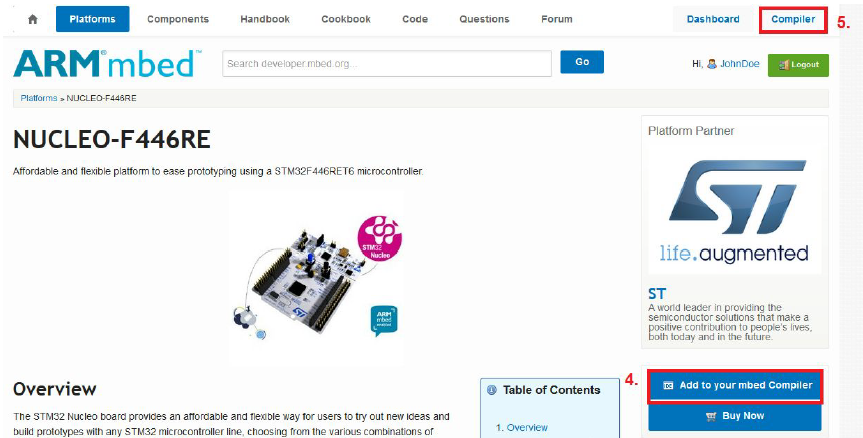
\includegraphics[width=0.9\textwidth]{figures/mbed-compiler.png}
\end{figure}

\subsection{Sample programs and binary upload to the device}

Click on ``New" in the top left corner (1.). In the pop-up window (2.) select the appropriate device type, and then we can select from one of the existing sample projects (or alternatively create a new one) and give a name for it. With the tick-box in the bottom we can select whether to update our code if one of the dependent libraries are updated. Click on OK and afterwards the newly created program will be visible under the My Programs section with the chosen name.
\begin{figure}[H]
    \centering
    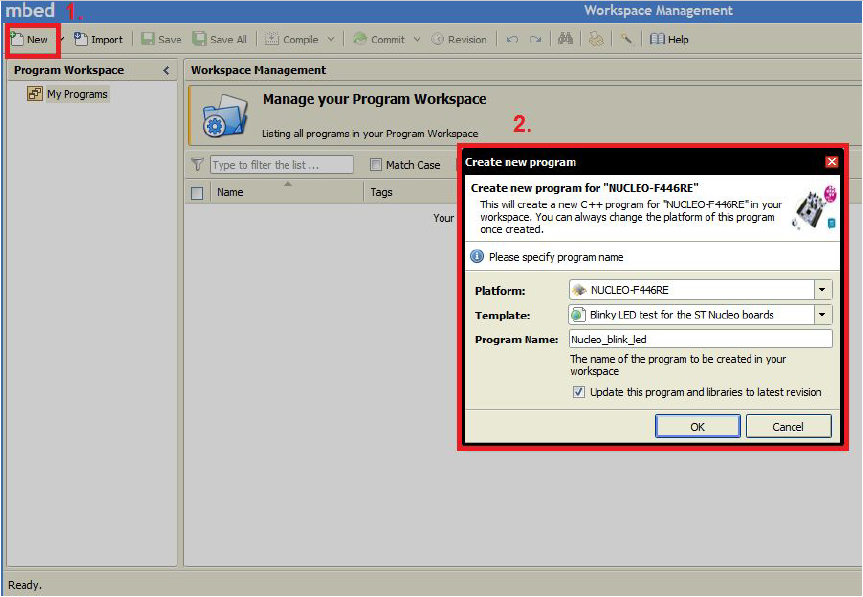
\includegraphics[width=0.9\textwidth]{figures/mbed-new.png}
\end{figure}

We can open and edit (1.) the source file by clicking on it in the left pane. As soon as we are done with the modifications the compilation can be started by clicking on ``Compile" button (2.). If there were no errors and the program compiles successfully the result will be file download pop-up for the resulting binary (3.)

\begin{figure}[H]
    \centering
    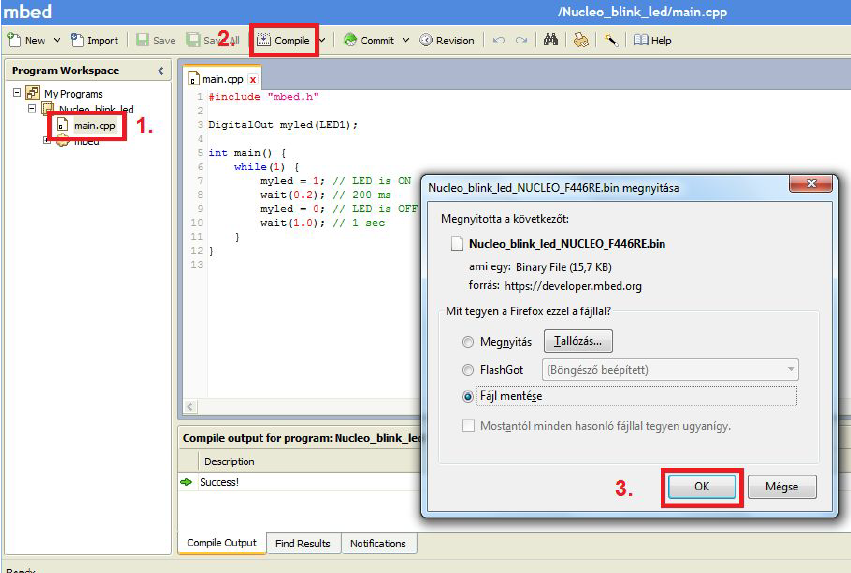
\includegraphics[width=0.9\textwidth]{figures/mbed-compile.png}
\end{figure}

Download/save this binary on the volume created by the dev board (NUCLEO). The green LED will start blinking during software upload to the micro-controller. If there are no errors our code will run on the device.

\begin{figure}[H]
    \centering
    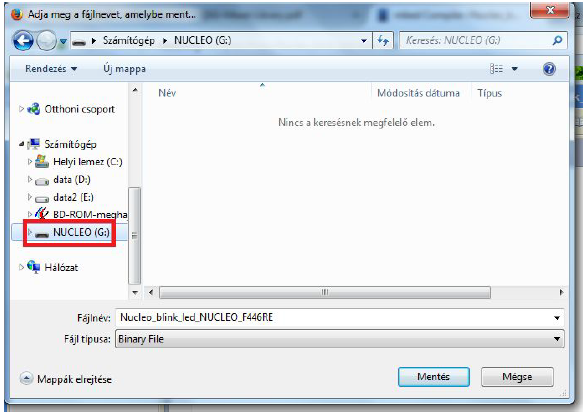
\includegraphics[width=0.9\textwidth]{figures/mbed-nucleo-save.png}
\end{figure}

\subsection{Creating an empty project}
Similarly to the previous steps click on ``New" (1.) then select "Empty Program" option (2.). Name the project (3.) then click OK. (4.)

\begin{figure}[H]
    \centering
    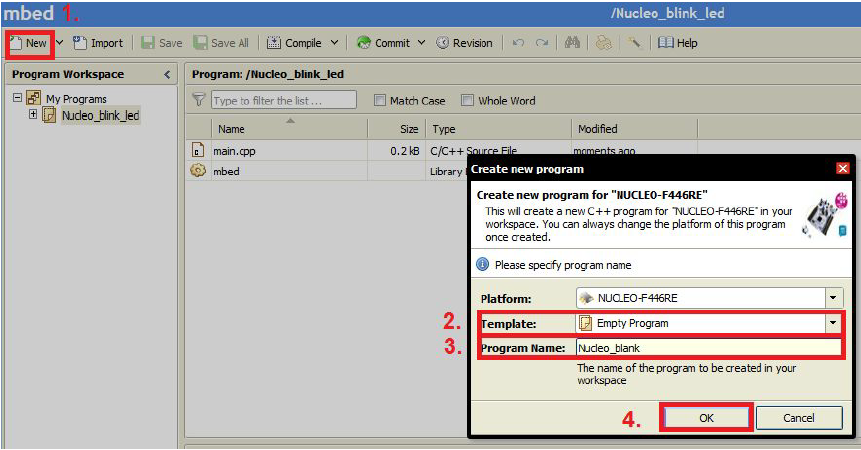
\includegraphics[width=0.9\textwidth]{figures/mbed-empty-proj.png}
\end{figure}

The empty application project needs at least the mbed runtime library that can be added to the project in the following way:
\begin{enumerate}
  \setcounter{enumi}{0}
  \item Select the project
  \item click on ``Import"
  \item select the ``Libraries" tab
  \item search for the word ``mbed"
  \item Import
\end{enumerate}

\begin{figure}[H]
    \centering
    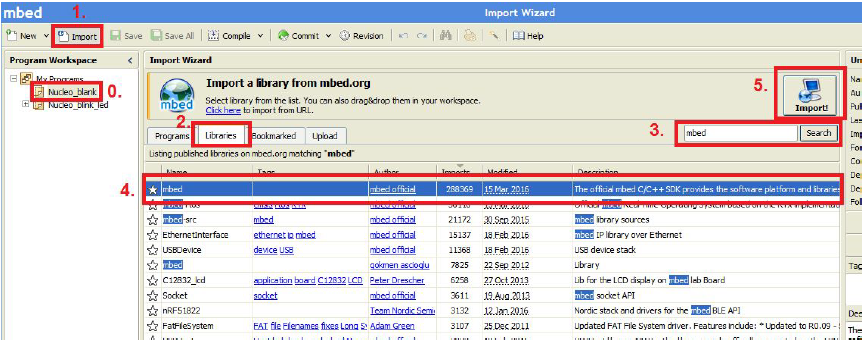
\includegraphics[width=0.9\textwidth]{figures/mbed-import.png}
\end{figure}

\subsection{Ways of importing}

There are some other ways for importing programs and libraries. A program can be imported based on the above describe method but selecting the ``Programs" tab (1.).
A program or library can be either uploaded from our local machine from a file (2.) or we can download it given that the url of it is know and we have sufficient privileges.

\begin{figure}[H]
    \centering
    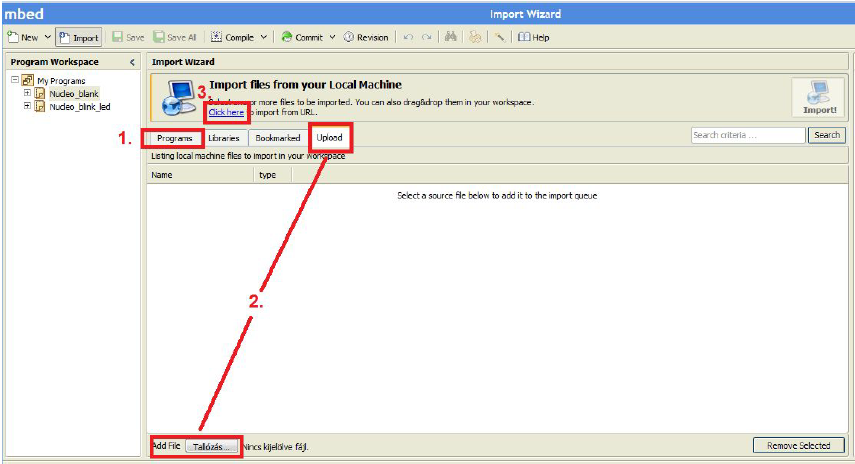
\includegraphics[width=0.9\textwidth]{figures/mbed-import2.png}
\end{figure}

In case if we are a part of a development team there is an option for importing the sources published by other developers.

\begin{figure}[H]
    \centering
    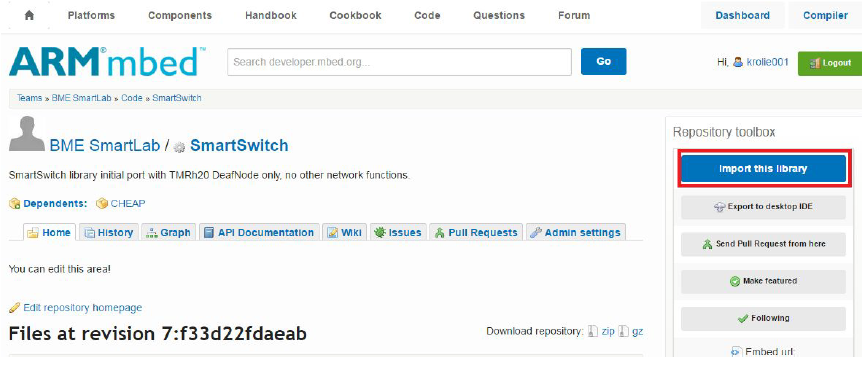
\includegraphics[width=0.9\textwidth]{figures/mbed-online-import.png}
\end{figure}
\begin{figure}[H]
    \centering
    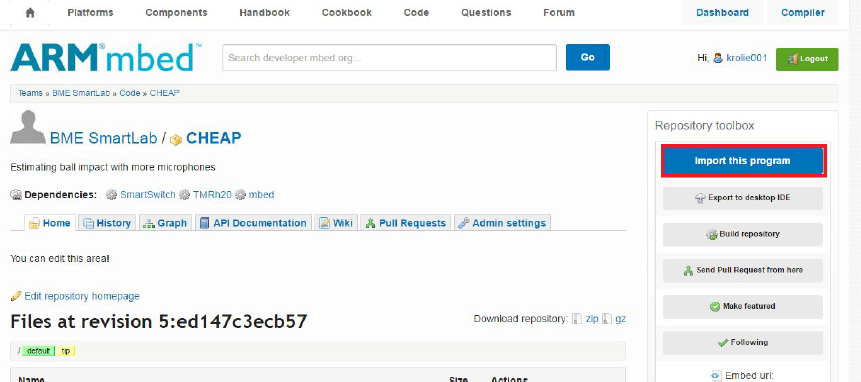
\includegraphics[width=0.9\textwidth]{figures/mbed-online-import2.png}
\end{figure}


\section{Further Reading}

\begin{itemize}
    \item \href{https://qosip.tmit.bme.hu/foswiki/pub/Meres/OpenFlowMScMeresiSegedlet/a19-lantz.pdf}{A Network in a
              Laptop: Rapid Prototyping for Software-Defined Networks}
    \item

          \href{https://qosip.tmit.bme.hu/foswiki/pub/Meres/OpenFlowMScMeresiSegedlet/mininet-hotnets2010-final.pdf}{Presentation
              of conference proceedings on Mininet}
    \item	Mininet page: \url{http://mininet.org/}
    \item	Mininet wiki: \url{https://github.com/mininet/mininet/wiki}
    \item	Mininet introduction: \url{https://github.com/mininet/mininet/wiki/  Introduction-to-Mininet}
    \item	Mininet Python API: \url{http://mininet.org/api/hierarchy.html}
\end{itemize}

OpenFlow specifications:
\begin{itemize}
    \item
          \href{https://qosip.tmit.bme.hu/foswiki/pub/Meres/OpenFlowMScMeresiSegedlet/openflow-spec-v1.0.0.pdf}{v1.0}
    \item
          \href{https://qosip.tmit.bme.hu/foswiki/pub/Meres/OpenFlowMScMeresiSegedlet/openflow-spec-v1.1.0.pdf}{v1.1}
    \item

          \href{https://qosip.tmit.bme.hu/foswiki/pub/Meres/OpenFlowMScMeresiSegedlet/openflow-switch-v1.3.4.pdf}{v1.3.4}
    \item

          \href{https://qosip.tmit.bme.hu/foswiki/pub/Meres/OpenFlowMScMeresiSegedlet/openflow-switch-v1.4.1.pdf}{v1.4.1}
    \item

          \href{https://qosip.tmit.bme.hu/foswiki/pub/Meres/OpenFlowMScMeresiSegedlet/openflow-switch-v1.5.1.pdf}{v1.5.1}

\end{itemize}

\appendix

\section{Entry quiz sample questions}

\begin{enumerate}
    \item Describe briefly the main concept of the OpenFlow recommendation.
    \item What are the components of an OpenFlow network?
\end{enumerate}

\section{Lab exercises}

\subsection{Lab environment}

\end{document}